
%%% Local Variables: 
%%% mode: latex
%%% TeX-master: "paper"
%%% End: 


We define a set of \emph{local} formulae. A formula is local if its groundings relate any number of observed ground atoms to exactly one hidden ground atom. For example, a grounding of the local formula 
\[lemma(p,+l_1) \wedge lemma(a,+l_2) \Rightarrow hasRole(p,a)\]
can be seen in the Markov Network of Figure \ref{fig:local2}. It connects a hidden \emph{hasRole} ground atom to two observed \emph{lemma} ground atoms. Note that the ``+'' prefix for variables indicates that there is a different weight for each possible pair of lemmas $(l_1,l_2)$.


\begin{figure}
\begin{center}
    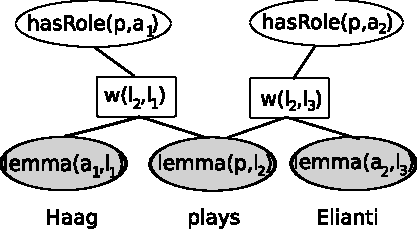
\includegraphics[scale=.70]{LocalFormula2}
\end{center}
\caption{Factor graph for the local formula in section \ref{sec:local}.}
\label{fig:local2}
\end{figure}


For the \emph{hasRole} and \emph{role} predicates we defined local formulae that aimed to reproduce the standard features used in previous work~\citep{xue04calibrating}. This also required us to develop dependency-based versions of the constituent-based features such as the syntactic path between predicate and argument, as proposed by \cite{xue04calibrating}. 

The remaining hidden predicates, \emph{isPredicate}, \emph{isArgument} and \emph{sense}, have local formulae that relate their ground atoms to properties of a contextual window around the token the atom corresponds to. For this we used the information provided in the closed track training corpus of the shared task (i.e. both versions of lemma and POS tags plus a coarse version of the POS tags). 

Instead of describing the local feature set in more detail we refer the reader 
to our MLN model files. 
\footnote{\url{http://thebeast.googlecode.com/svn/mlns/conll09}} They can be 
used both as a reference and as input to our Markov Logic 
Engine\footnote{\url{http://thebeast.googlecode.com}}, and thus allow the reader 
to easily reproduce our results. We believe that this is another advantage of 
explicitly separating model and algorithms by using first order probabilistic 
logic languages.

